\subsection{Problem Set 2}
    \begin{problem}[]
        Let $T = S^{1} \times S^{1}$ be the torus and
        $i \colon D^2 \hookrightarrow T$ and embedding of
        the unit disk that is disjoint from $S^{1}\times 
        \left\{ s_0 \right\} $. Define
        $A := \left( S^{1} \times \left\{ s_0 \right\}  \right) 
        \cup i \left( S^{1} \right) \subset T$.
        Let $x_0 = \left( s_0,s_0 \right) $ and
        $x_1 \in i \left( S^{1} \right) $.
        \begin{enumerate}
            \item Draw a picture of $\left( X,A \right) $ 
                and the two points $x_0$ and $x_1$.
            \item Construct an explicit bijection of
                sets
                $\pi_1 \left( T,A,x_1 \right) \cong
                \mathbb{Z}^2 \sqcup \mathbb{Z}$.
            \item Compute the relative homotopy groups
                $\pi_2 \left( T,A,x_0 \right) $ and
                $\pi_2 \left( T,A,x_1 \right) $.
        \end{enumerate}
    \end{problem}

    \begin{solution}
        (1) 
        \begin{figure}[htpb]
            \centering
            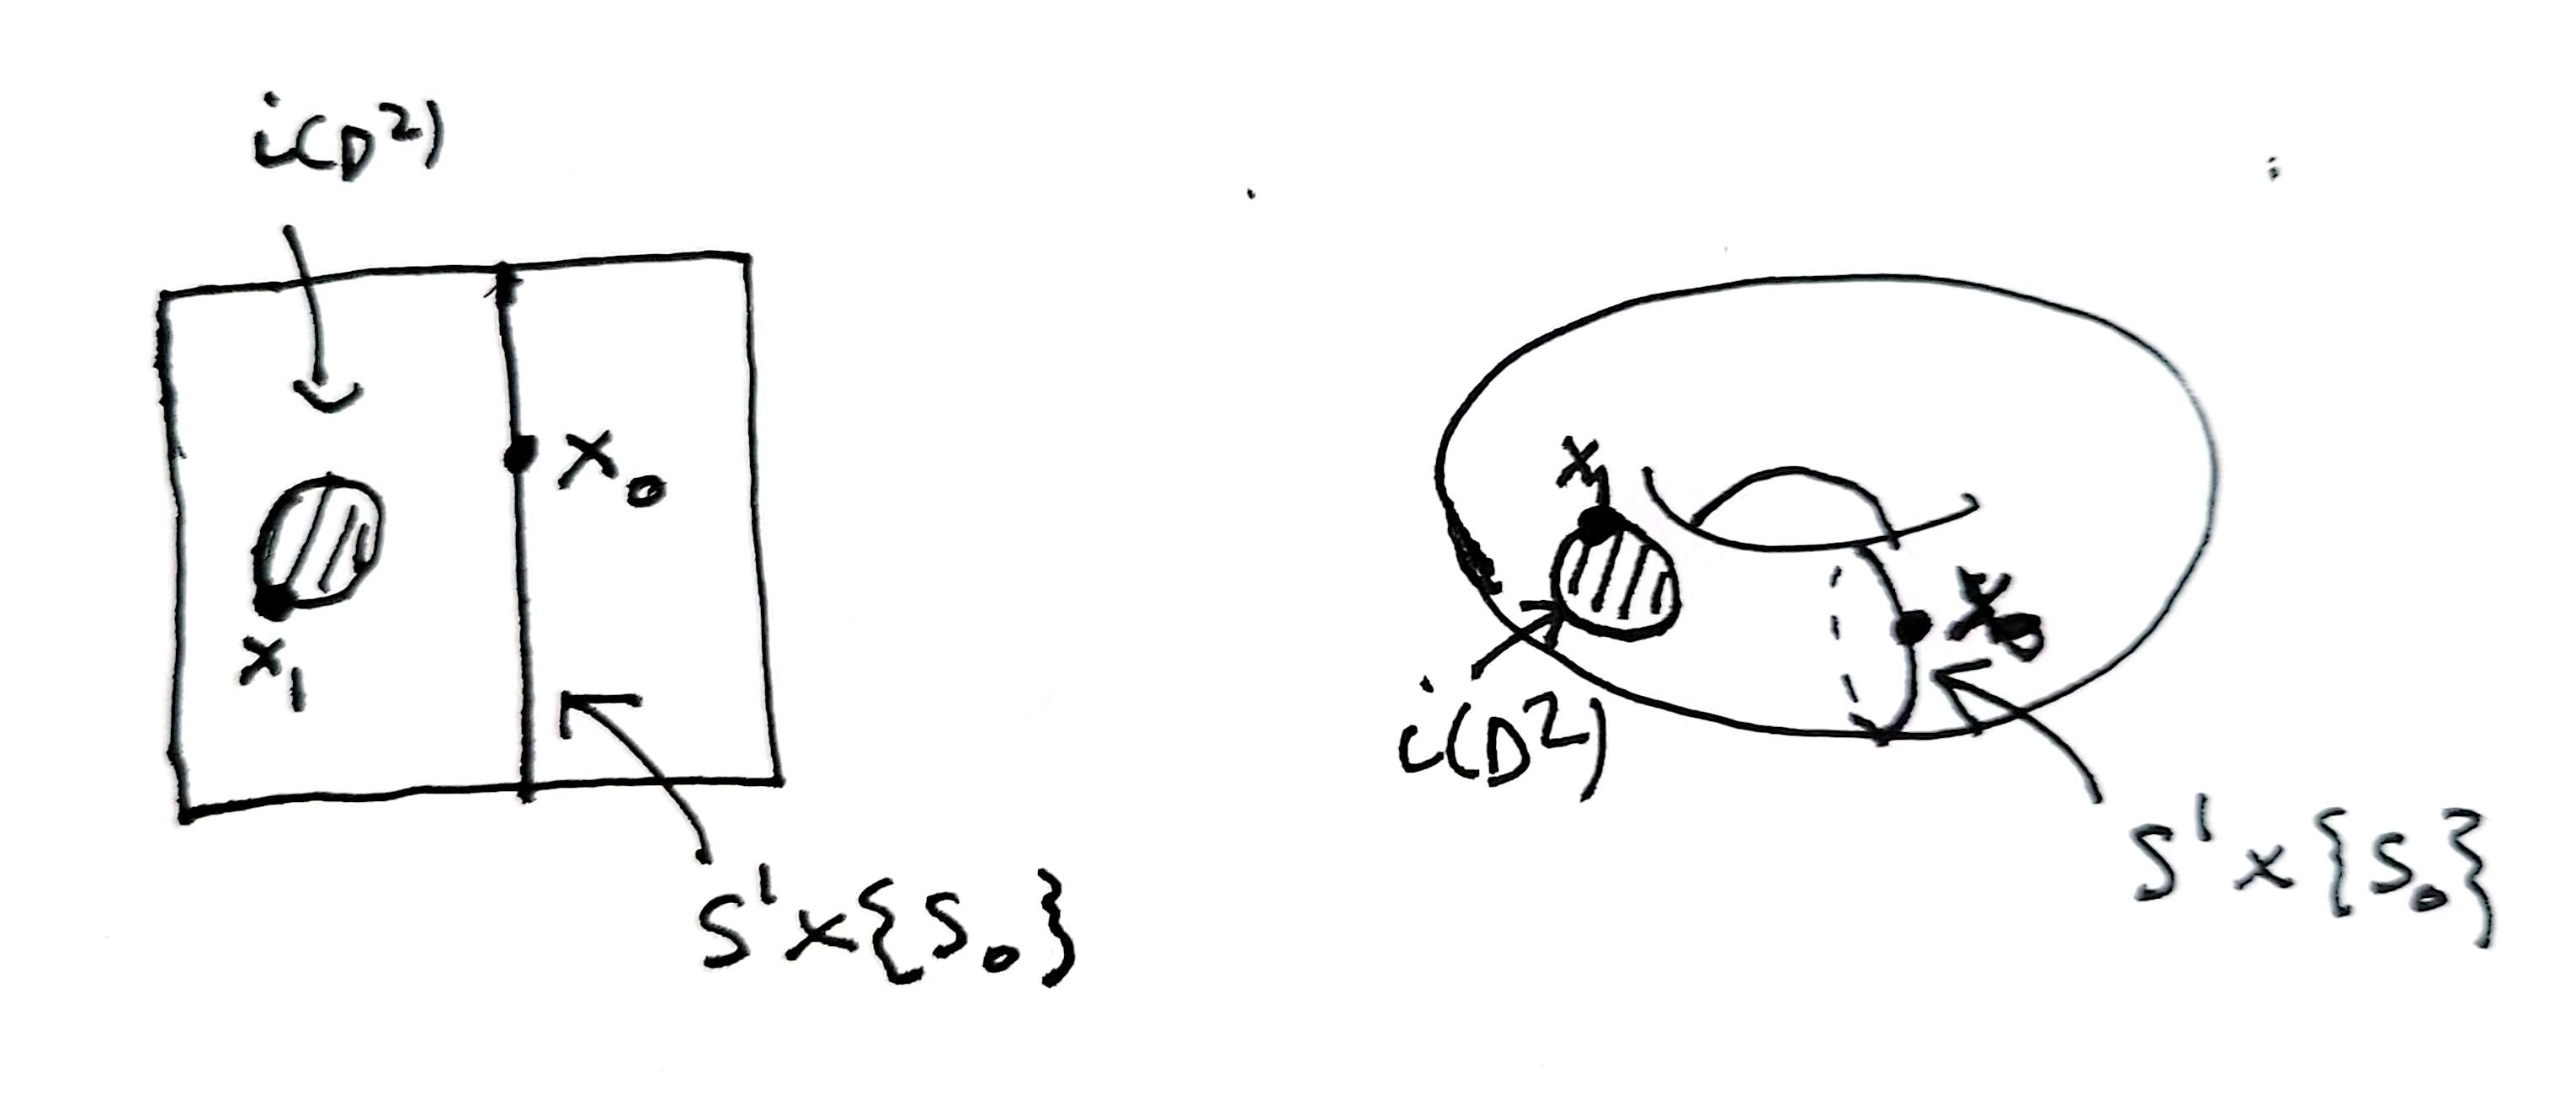
\includegraphics[width=0.8\textwidth]{Figures/p11.jpeg}
            \caption{Note that 
            in this figure, $A$ are the parts drawn
        without the interior of the disk $i(D^2)$.}
            \label{fig:p11-jpeg}
        \end{figure}

        (2)
        Recall that
        \[
        \pi_n (T,A,x_1) =
        \left[ I^{n},\partial I^{n},
        J^{n-1}; T,A, x_1 \right] .
        \] 
        Thus $\pi_1 \left( T,A,x_1 \right) $ becomes
        the set of homotopy classes
        of maps
        $\left( I, \left\{ 0,1 \right\} , \left\{ 1 \right\} 
        \right) \to \left( T,A,x_1 \right)$. That is, the
        set of paths in $T$ starting at a point in $A$ and
        ending at $x_1$ up to homotopy through such paths.\\
        For any map
        $ f \colon \left( I, \left\{ 0 \right\} , \left\{ 1 \right\} 
        \right) \to \left( T, A, \left\{ x_1 \right\}  \right) $, 
        can lift this to the universal cover since
        $I$ is simply connected. Let
        $\tilde{f} \colon 
        \left( I, \left\{ 0 \right\} , \left\{ 1 \right\}  \right) 
        \to \left( \mathbb{R}^2, 
        p^{-1} (A) , p^{-1}\left( \left\{ x_1 \right\}  \right) 
    \right) $.
    Now, $p^{-1}(A)$ can be visualized as
    tiling $\mathbb{R}^2$ by tiles
    as the left picture in Figure \ref{fig:p11-jpeg}, each
    tile of course contains precisely one
    element of the fiber $p^{-1}\left( 
    \left\{ x_1 \right\} \right) $. For the lift
    $\tilde{f}$, we choose a base point
    $\tilde{x_1}$ in
    $p^{-1}\left( \left\{ x_1 \right\}  \right) $. By
    the lifting theorem, there now exists
    a unique lift, call it $\tilde{f} \colon
    \left( I, \left\{ 1 \right\} 
    \right) \to \left( \mathbb{R}^2, 
    \left\{ \tilde{x_1} \right\} \right) $, such that
    $f = p \circ \tilde{f}$. Now,
    $f(0) \in A$ is the only condition, so
    $\tilde{f}(0)$ lies in $p^{-1}(A)$.
    Homotopies through maps which
    start in $A$ for $f$ correspond in the universal cover
    to letting $\tilde{f}(0)$ run freely through its
    path component in $p^{-1}(A)$. We can
    construct a bijection
    $\pi_0 \left( p^{-1}(A) \right) \cong 
    \mathbb{Z}^2 \sqcup \mathbb{Z}$ by
    identifying the component of
    $p^{-1} \left( i \left( S^{1} \right)  \right) \cap
    \left[ n,n+1 \right] \times \left[ m,m+1 \right] $ with
    $\left( n,m \right) \in \mathbb{Z}^2$ and
    identifying the
    vertical line in
    $p^{-1}\left( S^{1} \times \left\{ s_0 \right\}  \right) 
    \cap [n,n+1)$ with $n \in  \mathbb{Z} \subset 
    \mathbb{Z}^2 \sqcup \mathbb{Z}$. This is obviously bijective.
    We can always homotopy $f$ to be a straight-line in
    the universal cover, so the only thing that determines
    the equivalence class of
    $f$, given that $\tilde{f}$ ends at $\tilde{x_1}$,
    is which path component in
    $\mathbb{Z}^2 \sqcup \mathbb{Z}$ it start in.
    This gives an injective map
    $\varphi \colon \pi_1 \left( T,A,x_1 \right) 
    \to \mathbb{Z}^2 \sqcup \mathbb{Z}$.
    To see that it is surjective, it is clear that
    choosing $\tilde{x_1}$ as above and
    choosing any point in the path component corresponding to
    an element $x \in \mathbb{Z}^2 \sqcup \mathbb{Z}$, taking
    the straight line between these two points gives
    a path $\tilde{f} \colon I \to \mathbb{R}^2$ 
    such that $f := p \circ \tilde{f} $ gives a path
    $\left[ f \right] \in \pi_1 \left( T,A,x_1 \right) $,
    and, by construction,
    $\varphi (\left[ f \right] ) = x$.

    Thus $\pi_1 (T,A,x_1) \cong \mathbb{Z}^2 \sqcup \mathbb{Z}$.



        (3) Let
        $\iota \colon A \to T$ be the inclusion.
        Then using the LES of relative homotopy groups, we
        have that 
        \begin{align*}
            \pi_2 (T,x_i)
            \to \pi_2 \left( T,A, x_i \right) 
            \to \pi_1 \left( A,x_i \right) \stackrel{\iota_*}{\to} 
            \pi_1 \left( T,x_i \right) 
        \end{align*}
        is exact for $i = 0,1$.
        For $i=0,1$, 
        $\pi_1 (A,x_i) \cong \mathbb{Z}$ and
        $\pi_1 (T,x_i) \cong \mathbb{Z}^2$, while
        $\pi_2 \left( T,x_i \right) \cong
        \pi_2 \left( S_1 \right) \times 
        \pi_2 \left( S^{1} \right) \cong 1$ for
        both $i=0,1$.
        Hence
        $\pi_2 \left( T,A,x_i \right) \cong
        \ker \iota_*$.
        First, suppose $i = 0$. 
        Then $\iota$ induces the map
        $\mathbb{Z} \cong \pi_1 \left( A, x_0 \right) 
        \to \pi_1 \left( T, x_0 \right) \cong \mathbb{Z}^2$ 
        given by
        $n \mapsto \left( 0,n \right) $, so
        $\ker \iota_*$ is trivial in this case, so
        $\pi_2 \left( T, A, x_0 \right) \cong 0$.
        Suppose now that $i = 1$. Then
        any loop in the image of $\iota_*$ is clearly
        based nullhomotopic by contracting 
        $i(D^2)$ to the point $x_1$. Thus
        $\ker \iota_* =
        \pi_1 \left( A, x_1 \right) 
        \cong \pi_1 (S^{1}) \cong \mathbb{Z}$.
        So $\pi_2 \left( T,A,x_1 \right) \cong
        \mathbb{Z}$.
    \end{solution}


    \begin{problem}[]
        \begin{enumerate}
            \item Compute $\pi_1 \left( S^{1} \vee
                S^2\right) $ and describe the universal
                cover of $S^{1} \vee S^2$.
            \item Show that $\pi_2 \left( S^{1} \vee
                S^2 \right) $ is isomorphic
                to $\bigoplus_{\mathbb{Z}} \mathbb{Z}$.
            \item Explicitly describe the action of
                $\pi_1 \left( S^{1} \vee S^2 \right) $ on
                $\bigoplus_{\mathbb{Z}} \mathbb{Z} \cong
                \pi_2 \left( S^{1} \vee S^2 \right) $.
        \end{enumerate}
    \end{problem}

    \begin{solution}
        (1) 
        The universal cover of $S^{1} \vee S^2 =: X$, which
        we will denote $\tilde{X}$, is
        clearly
        $\mathbb{R}$ with a copy of $S^2$ attached to
        each integer of $\mathbb{R}$.\\
        Let 
        $A_1$ be the $S^{1}$ part
        together with a small open neighborhood
        of the base point in $S^2$, and
        likewise, $A_2$ be $S^2$ together with a small
        open neighborhood of the base point in $S^{1}$ - here
        the base points are the points that get identified
        in the construction of $S^2 \vee S^{1}$.
        Applying van Kampen, we find that
        $\pi_1 \left( S^2 \vee S^{1} \right) 
        \cong \pi_1 \left( S^{1} \right) * \pi_1\left( S^2 \right) 
        / N$ where $N$ is generated
        by all elements of the form
        $i_{12}(w) i_{21}(w)^{-1}$ for
        $w \in \pi_1 \left( A_1 \cap A_2 \right) $.
        But $A_1 \cap A_2$ is contractible, so
        $N \cong 0$. Since $\pi_1 \left( S^{1} \right) \cong
        \mathbb{Z}$ and $\pi_1 \left( S^2 \right) \cong 0$, 
        we conclude that $\pi_1 \left( S^{2} \vee S^{1}  \right) 
        \cong \mathbb{Z}$.\\
        \linebreak
        (2) To compute
        $\pi_2 \left( S^{1} \vee S^2 \right) $, it suffices
        to compute $\pi_2$ of its universal cover since
        these are isomorphic. The universal cover
        is $\mathbb{R}$ with $S^2$ attached at each integer.
        Since $\mathbb{R} \simeq \left\{ * \right\}$, the
        universal cover is homotopy equivalent to
        $\vee_{\mathbb{Z}} S^2$ for example by
        using proposition 0.16 and 0.17 in Hatcher.\\
        Since homotopy groups are invariant under based homotopy
        equivalences, it suffices to
        compute $\pi_2 \left( \bigvee_{\mathbb{Z}}S^{2} \right) $.\\
        But $\bigvee_{\mathbb{Z}}S^2$ is $1$-connected,
        so if $\tilde{H}_2 \left( \bigvee_{\mathbb{Z}}S^2 \right) 
        \cong H_2 \left( \bigvee_{\mathbb{Z}}S^2 \right) $ 
        is nonzero, then by the Hurewicz theorem,
        we will obtain that 
        $\pi_2\left( \bigvee_{\mathbb{Z}}S^2 \right) 
        \cong H_2 \left( \bigvee_{\mathbb{Z}}S^2 \right) $.
        Now, we can give
        $\bigvee_{\mathbb{Z}}S^2$ a $\Delta$-complex (or
        cellular) structure
        with a single $0$-simplex
        and a $2$-simplex for each
        $S^2$ in $\bigvee_{\mathbb{Z}}S^2$. The
        associated simplicial chain complex then becomes
        \[
        \ldots \to 0 \to \bigoplus_{\mathbb{Z}}\mathbb{Z}
        \to 0 \to \mathbb{Z} \to 0 \to \ldots
        \] 
        with $0$ everywhere else. In particular then
        $H_2 \left( \bigvee_{\mathbb{Z}}S^2 \right) 
        \cong \oplus_{\mathbb{Z}}\mathbb{Z}$ since there
        cannot be any cancellation from the
        maps.
        Since the Hurewicz isomorphism 
        takes 
        $f \in \pi_2 \left( \bigvee_{\mathbb{Z}} S^2 \right) $,
        to $f_* \left[ 1 \right] \in 
        H_2 \left( \bigvee_{\mathbb{Z}}S^2 \right) $ 
        for $\left[ 1 \right] \in H_2\left( S^2 \right) $ 
        a generator, we find that through our proof
        using the $\Delta$-complex of $\bigvee_{\mathbb{Z}}S^2$,
        we found that the inclusions
        $S^2 \hookrightarrow \bigvee_{\mathbb{Z}}S^2$ 
        in fact induce generators on homology: i.e.,
        the images of the different inclusions
        $\iota_i \colon H_2 \left( S_i^2 \right) 
        \hookrightarrow H_2 \left( \bigvee_{i \in \mathbb{Z}}
        S_i^2 \right) 
        \cong \bigoplus_{\mathbb{Z}}\mathbb{Z}$ generate
        $\bigoplus_{\mathbb{Z}} \mathbb{Z}$, and hence
        also $\pi_2 \left( \bigvee_{\mathbb{Z}}S^2 \right) $ 
        under the Hurewicz isomorphism.\\
        \linebreak
        








    (3) 
    Recall that
    the action of $\pi_1 \left( S^{1} \vee S^2 \right) $ 
    on $\pi_n \left( S^{1} \vee S^{2} \right) $ 
    makes $\pi_n \left( S^{1} \vee S^2 \right) $ 
    into a $\mathbb{Z} \left[ \pi_1 \left( S^{1} \vee S^2 \right) 
    \right] $-module. We saw that
    $\pi_1 \left( S^{1} \vee S^2 \right) \cong \mathbb{Z}$. Let
    $\gamma$ be a loop that goes once around the $S^{1}$ factor.
    This generates $\pi_1 \left( S^{1} \vee S^2 \right) 
    \cong \mathbb{Z}$, so it suffices
    to describe the action of $\gamma$ on
    $\pi_2 \left( S^{1} \vee S^2 \right) $ since
    $\pi_2$ now becomes a $\mathbb{Z}\left[ \gamma \right] $-module
    under this action.
    Since also $\pi_2 \left( S^{1} \vee S^2 \right) 
    \cong \bigoplus_{\mathbb{Z}} \mathbb{Z}$, it
    suffices to describe the action of
    $\gamma$ on an arbitrary basis element
    of $\bigoplus_{\mathbb{Z}}\mathbb{Z}$, say,
    corresponding to the image under $p_*$ of
    some an inclusion of some $S^2 \hookrightarrow 
    \tilde{X}$. Suppose we choose the inclusion
    $\alpha$ into the $S^2$ attached to $1_n \in \mathbb{Z}_n$.\\
    Then $p_* \alpha = \left[ \eta_n \xi \right]
    = 1_{n} \in \mathbb{Z}_n$ where
    $\eta_n$ is the loop that winds around the $S^{1}$ factor
    $n$ times and $\xi$ is the inclusion
    $S^2 \hookrightarrow S^{1} \vee S^2$.\\
    In particular then
    $\gamma p_* \alpha = \left[ \eta_{n+1} \xi \right] 
    = 1_{n+1} \in \mathbb{Z}_{n+1}$.\\
    \linebreak
    This completes the description, but I will also
    give an alternative description just for
    completeness where I expound on some details
    between the homomorphisms
    $H_2 \left( \bigvee_{\mathbb{Z}}S^2 \right) 
    \cong \pi_2 \left( \bigvee_{\mathbb{Z}} S^2 \right) 
    \cong \pi_2 \left( S^{1} \vee S^2 \right) $ that underlies
    the above explanation. We will use the correspondence between
    the $\pi_1$ action on $\pi_n (X)$ and its action
    on $\pi_n \left( \tilde{X} \right)  $ where
    $\tilde{X}$ was the universal covering space.\\
    To this end, we have previously shown the following:
    \begin{lemma}[]
        Let $p \colon \tilde{X} \to X$ be the universal cover
        of a path-connected space $X$. Under
        the isomorphism $\pi_n (X) \cong \pi_n (\tilde{X})$, for
        $n\ge 2$, the action of $\pi_1 (X)$ on
        $\pi_n (X)$ corresponds to the action
        of $\pi_1(X)$ on $\pi_n \left( \tilde{X} \right) $ 
        induced by the action of $\pi_1 (X)$ on
        $\tilde{X}$ as deck transformations.
        More precisely,
        for $\gamma \in \pi_1 \left( X, x_0 \right) ,
        \alpha \in \pi_n \left( \tilde{X},
        \tilde{x}_0 \right) ,
        \tilde{\gamma}$  the lift of $\gamma$, and
        $\gamma_*$ the homomorphism induced
        by the action of $\gamma$ on $\tilde{X}$, we have
        $\gamma p_* \left( \alpha \right) =
        p_* \left( \beta_{\tilde{\gamma}} 
        \left( \gamma_* \left( \alpha \right)  \right) \right) $.
    \end{lemma}

    Let $\alpha \in \pi_2 \left( \tilde{X} \right) $  be
    the element corresponding under the isomorphism
    $\pi_2 (X) \cong \pi_2(\tilde{X})$ to the class
    of our chosen
    inclusion $S^2 \hookrightarrow \bigvee_{\mathbb{Z}}S^2$.
    That is, $\alpha$ is the inclusion of
    $S^2$ into one of the $S^2$ in the universal cover.
    To understand $\gamma p_* \left( \alpha \right) $, we
    can thus look at
    $p_* \left( \beta_{\tilde{\gamma}} 
    \left( \gamma_* \left( \alpha \right)  \right) \right) $.
    Now, $\gamma_* \left( \alpha \right) $ will
    simply be the inclusion of $S^2$ to 
    the $S^2$ "above" the previous one in the
    universal cover. So if we previously included our
    $S^2$ into the $S^2$ attached to
    $n \in \mathbb{R} \subset \tilde{X}$, then
    $\gamma_* \left( \alpha \right) $ corresponds to
    including $S^2$ into the $S^2$ attached to
    $n+1 \in \mathbb{R} \subset \tilde{X}$.
    Then $\beta_{\tilde{\gamma}}$ is simply the change-or-basepoint
    transformation depicted in the picture on
    page 341 in Hatcher. I.e., it essentially shrinks
    $\alpha$ and attaches it inside a larger square
    where we put $\tilde{\gamma}$ on each radial line
    in-between  the squares. 
    If we understand our isomorphism
    $\pi_2 \left( \bigvee_{\mathbb{Z}}S^2 \right) 
    \cong \bigoplus_{i \in \mathbb{Z}}\mathbb{Z}_i$ as
    the generator for $\mathbb{Z}_i$ corresponding under
    the Hurewicz isomorphism to the inclusion
    of $S^2$ into the sphere attached to $i \in \mathbb{Z}$,
    then we find that
    $\alpha \mapsto 
    \beta_{\tilde{\gamma}} \left( \gamma_* \left( \alpha \right) 
    \right) $ precisely sends $\alpha = 
    1_n \in \mathbb{Z}_n$ to $1_{n+1} \in \mathbb{Z}_{n+1}$. 
    Under $p_*$, this
    may be interpreted again as
    sending $1_{n} \mapsto 1_{n+1}$ when
    $n$ corresponds to $ \left[ \eta
    \xi \right]$ where
    $\eta$ is the loop that winds around the $S^{1}$ factor
    $n$ times and
    $\xi$ is the inclusion of $S^2 \hookrightarrow
    S^{1} \vee S^2$.
    \end{solution}


    \begin{problem}[]
        Let $\left( X,A,x_0 \right) $ be a pointed pair
        such that the inclusion
        $i \colon A \hookrightarrow X$ is based nullhomotopic
        (the nullhomotopy preserves the basepoint). The goal
        is to show that for $n\ge 2$, there is an isomorphism
        of groups:
        \[
        \pi_n (X,A,x_0) \cong \pi_n (X,x_0) \times 
        \pi_{n-1}(A,x_0).
        \] 
        \begin{enumerate}
            \item Show that there is an exact sequence
                of groups
                \[
                1 \to \pi_n (X,x_0) 
                \stackrel{j_*}{\to} 
                \pi_n \left( X, A, x_0 \right) 
                \stackrel{\partial_*}{\to} 
                \pi_{n-1}(A,x_0) \to 1.
                \] 
            \item Using a based nullhomotopy
                $H \colon A \times \left[ 0,1 \right] 
                \to X$, construct a natural group morphism
                \[
                r_* \colon \pi_n (X,A,x_0) \to 
                \pi_n (X,x_0)
                \] 
                such that $r_* \circ j_* = 1$.
            \item Show that for any short exact sequence
                of groups
                \[
                1 \to A \stackrel{\alpha}{\to} 
                B \stackrel{\beta}{\to} C \to 1
                \] 
                such that $\alpha$ admits a retraction, there
                is a group isomorphism
                \[
                B \cong A \times C.
                \] 
                Conclude the desired isomorphism.
        \end{enumerate}
    \end{problem}

    \begin{proof}
        (1) From the LES for relative homotopy groups, we obtain that
        \[
        \pi_n (A, x_0) \stackrel{i_*}{\to}  \pi_n(X,x_0)
        \stackrel{j_*}{\to} \pi_n \left( X, A, x_0 \right) 
        \stackrel{\partial_*}{\to} 
        \pi_{n-1}(A,x_0) \stackrel{i_*}{\to} 
        \pi_{n-1} \left( X, x_0 \right) 
        \] 
        is exact.
        For $n\ge 2$, all the sets in the exact sequence are
        groups and the maps are group homomorphisms.
        Since homotopic maps relative to the base point induce
        the same maps on homotopy groups, we find by assumption
        that $i_* = 0$. Therefore,
        \[
        1 \stackrel{0}{\to}   \pi_n(X,x_0)
        \stackrel{j_*}{\to} \pi_n \left( X, A, x_0 \right) 
        \stackrel{\partial_*}{\to} 
        \pi_{n-1}(A,x_0) \stackrel{0}{\to} 
        1
        \] 
        is exact.\\
        \linebreak
        (2) Let
        $\left[ f \right] \in \pi_n \left( X, A,x_0 \right) $
        and consider a representative
        $f \colon \left( D^{n}, S^{n-1},
        s_0 \right) \to 
        \left( X,A,x_0 \right) $.
        We put $f$ on the bottom of a cylinder
        $D^{n} \times \left\{ 0 \right\} \subset 
        D^{n} \times I$.
        Now $H \left( f(x),t \right) $ 
        gives a homotopy
        $S^{n-1} \times I \to X$, so we
        can use this on 
        $S^{n-1} \times I \subset 
        D^{n} \times I$ of the cylinder.
        Now we use that
        $D^{n} \times \left\{ 0 \right\} 
        \cup S^{n-1} \times I \cong
        D^{n}$ (see Figure \ref{fig:p31-jpeg}). 
        Denote this
        homeomorphism by $\varphi 
        \colon D^{n} \to D^{n} \times \left\{ 0 \right\} \cup 
        S^{n-1} \times I$.

        \begin{figure}[htpb]
            \centering
            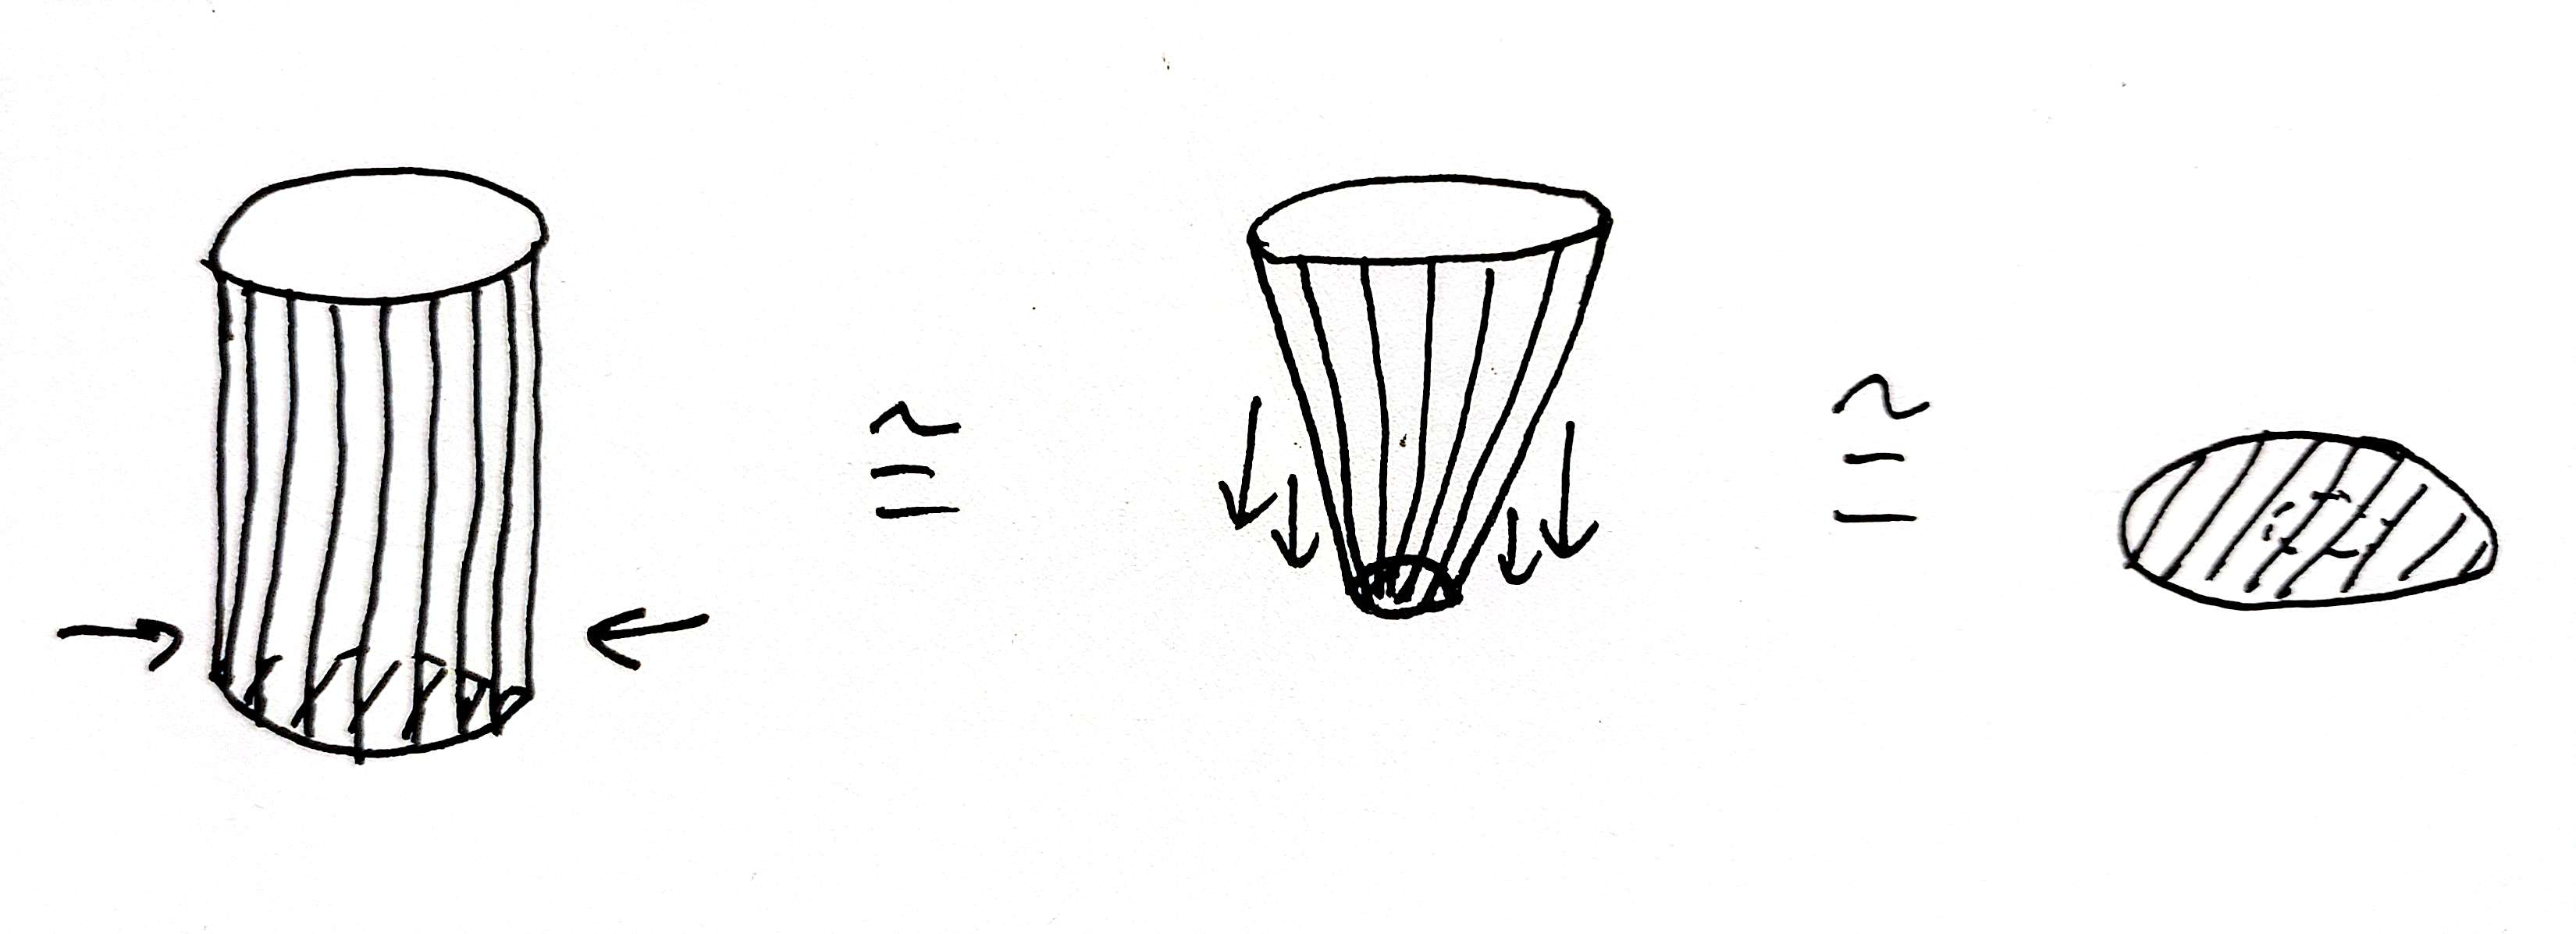
\includegraphics[width=0.8\textwidth]{Figures/p31.jpeg}
            \caption{}
            \label{fig:p31-jpeg}
        \end{figure}

        Define
        $h \colon S^{n-1} \times I$ by
        $h(x,t ) = H\left( f(x), t \right) $ and
        define $h \cup f \colon
        D^{n} \times \left\{ 0 \right\} \cup 
        S^{n-1} \times I$ by
        $f$ on $D^{n} \times \left\{ 0 \right\} $ and
        $h$ on $S^{n-1} \times I$. Then define
        $h \cup f \circ \varphi \colon
        D^{n} \to X$.
        Now $h \cup f \circ \varphi $ maps
        $\partial D^{n}$ to
        $x_0$, so
        it factors through the quotient
        $D^{n} \to S^{n}$ and induces
        a map
        $ \Gamma
        \colon \left( S^{n}, pt \right) 
        \to \left( X,x_0 \right) $, where
        $pt$ is the point that the boundary collapses to.
        This is well-defined since if
        $f \simeq f' \rel s_0$ through 
        a homotopy $F \colon D^{n} \times I \to X$, then
        $\tilde{h}(x,t,s) = 
        H\left( F(x,s), t \right) $ gives a map
        $S^{n-1} \times I \times I$ - and
        this homotopy is constant on the
        boundary $S^{n-1} \times \left\{ 1 \right\} $.
        Then taking
        $\tilde{h} \cup  F \colon
        \left( D^{n} \times \left\{ 0 \right\} 
        \cup S^{n-1} \times I\right)  \times I 
        \cong D^{n-1} \times \left\{ 0 \right\} \times I
        \cup S^{n-1} \times I \times I \to X$, we
        obtain a homotopy
        $\tilde{h}\cup F \circ \varphi \colon
        D^{n} \times I \to X$ which is constant on the
        boundary throughout, hence induces the desired
        homotopy $S^{n} \times I \to X$ between
        $\Gamma$ and $\Gamma' \rel \left\{ pt \right\} $.\\
        To see that it is a group morphism,
        see Figure \ref{fig:p32-jpeg}. Here
        the top left picture depicts
        $\Gamma$ obtained from
        $f + g \in 
        \pi_n \left( X, A, x_0 \right) $.
        The bottom left picture represents
        $\Gamma_f + \Gamma_g$, where
        $\Gamma_f$ is obtained from $f$ by the above procedure
        and $\Gamma_g$ is obtained from
        $g$ by the procedure. 
        Hence $r_* \left( \left[ f \right] +
        \left[ g \right] \right) 
        = r_* \left( \left[ f \right]  \right) 
        + r_* \left( \left[ g \right]  \right) $.

        \begin{figure}[htpb]
            \centering
            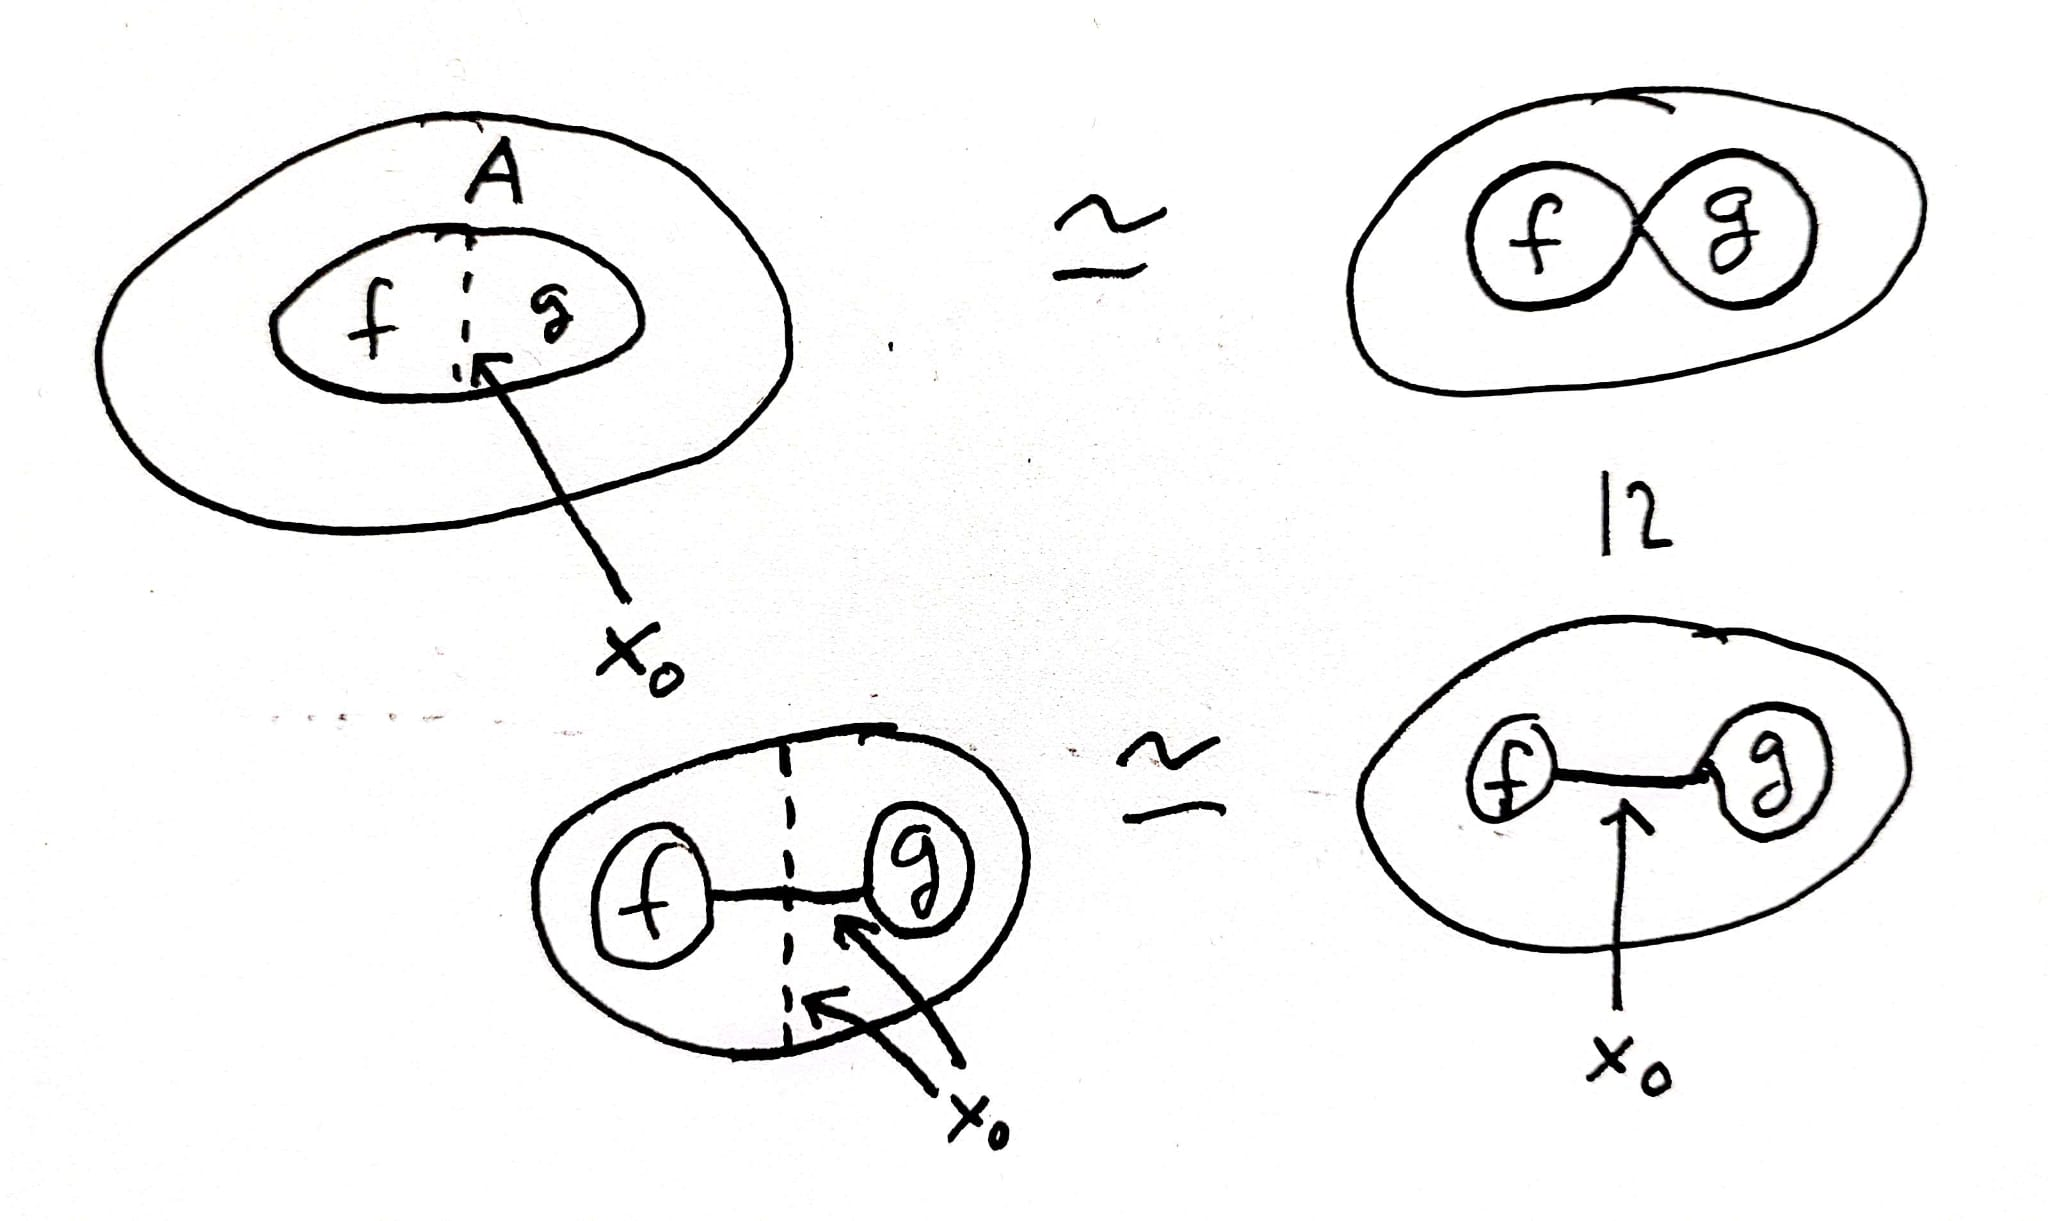
\includegraphics[width=0.7\textwidth]{Figures/p32.jpeg}
            \caption{}
            \label{fig:p32-jpeg}
        \end{figure}

        Naturality amounts to showing that 
        $r_*$ defines a natural transformation from
        $\pi_n \left( - , -, - \right) $ to
        $\pi_n (-,-)$ on the
        category of based pairs $\left( X,A \right) $ 
        such that $A \hookrightarrow X$ is
        based nullhomotopic. That is, that given
        a map  $f \colon \left( X, A, x_0 \right) 
        \to \left( Y,B,y_0 \right) $, with
        both $A \hookrightarrow X$ and
        $B \hookrightarrow Y$ based nullhomotopic, the diagram
        \begin{equation*}
        \begin{tikzcd}
            \pi_n \left( X,A,x_0 \right) \ar[r, "r_*"] \ar[d, "
            f_*"] &
            \pi_n (X,x_0) \ar[d, "f_*"] \\
            \pi_n \left( Y,B,y_0 \right) \ar[r, "r_*"] & 
            \pi_n (Y,y_0)
        \end{tikzcd}
        \end{equation*}
        commutes.

        Now, if $H \colon A \times I \to X$ is
        the based nullhomotopy
        of $A \hookrightarrow X$ and
        $G \colon B \times I \to Y$ is the based
        nullhomotopy of 
        $B \hookrightarrow Y$, then
        for $\left[ f \right] \in 
        \pi_n \left( X,A,x_0 \right) $, we get the
        situation of
        Figure \ref{fig:p33-jpeg}.
        In the central part, these maps agree - namely they
        are $f \circ g$. We are thus asking for
        a homotopy
        between
        $f \circ H \left( g(x),t \right) $ and
        $G\left( f \circ g(x), t \right) $. So
         we want a map
         $L \colon S^{n-1} \times I \times I \to X$. 
         We may assume without loss of generality
         that $H$ and $G$ map
         $S^{n-1} \times \left\{ 0 \right\} $ to
         $x_0$ and $y_0$, respectively, instead
         of $S^{n-1} \times \left\{ 1 \right\} $.
         Now we let $L$ be
         given by
         \[
         L \left( x, t, s \right) 
         \begin{cases}
             f \circ H\left( g(x), (1-2s) t \right) ,& 
             s \in \left[ 0,\frac{1}{2} \right] \\
             G \left( f \circ g(x), 2s-1 \right),& s 
             \in \left[ \frac{1}{2},1 \right].
         \end{cases}
         \] 
         This gives naturality.

        \begin{figure}[htpb]
            \centering
            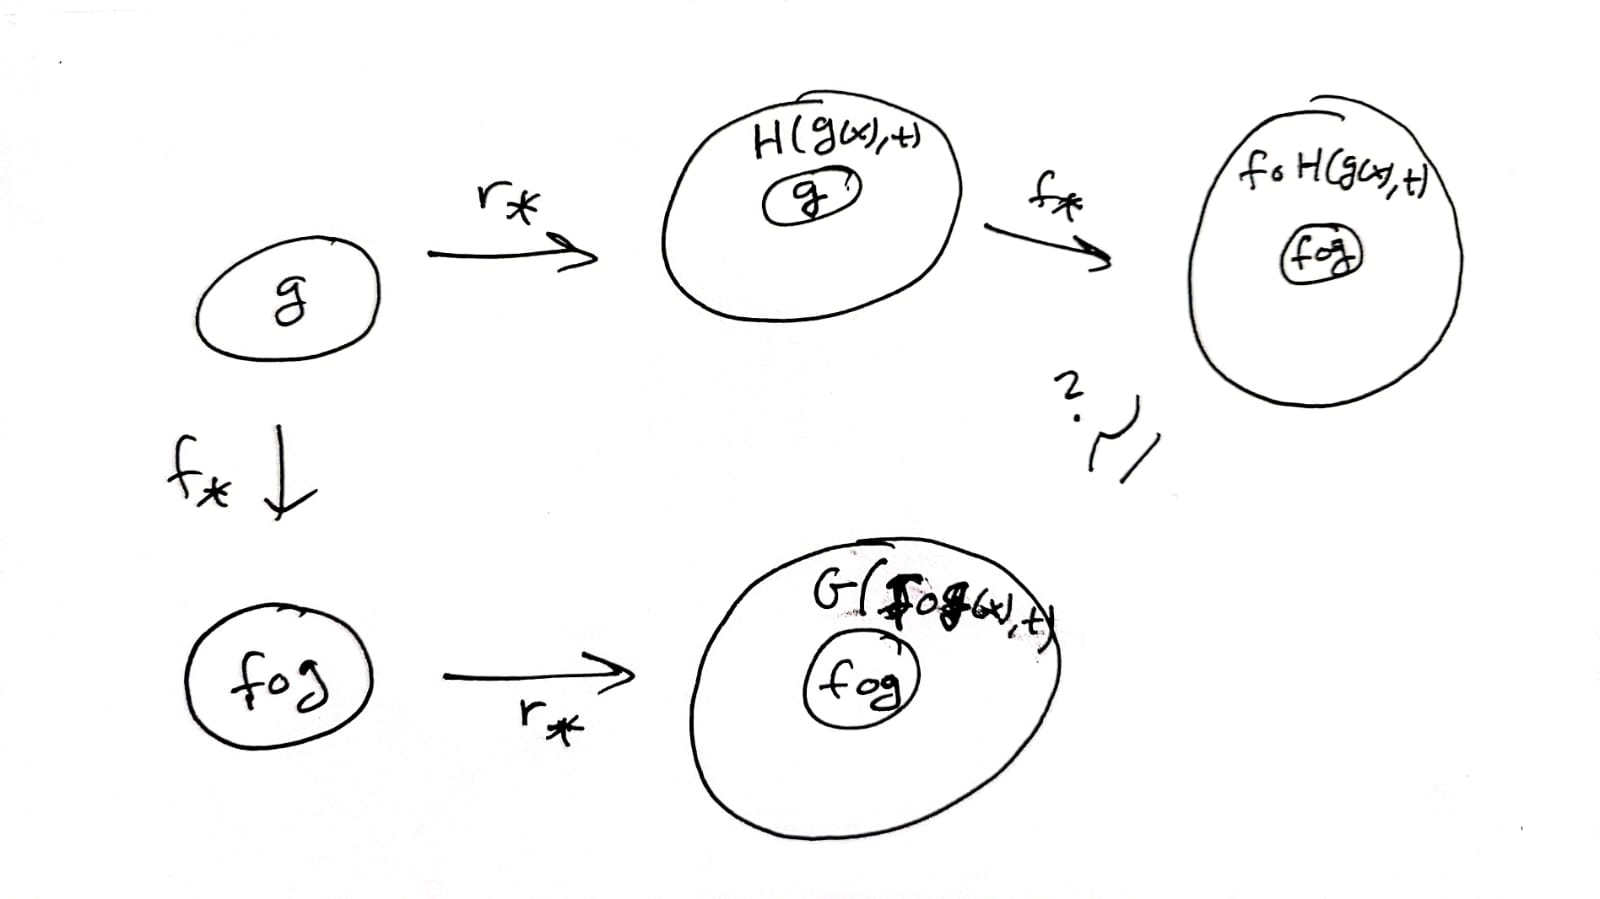
\includegraphics[width=0.8\textwidth]{Figures/p33.jpeg}
            \caption{}
            \label{fig:p33-jpeg}
        \end{figure}
        





        Now, for 
        $\left[ f \right]  \in \pi_n \left( X, x_0 \right) $,
        we have that the boundary is
        already mapped to $x_0$, so
        $H \left( f(x), t \right)$ is constant
        on $S^{n-1} \times I$ since
        $H$ is relative the basepoint. Hence
        $\Gamma \simeq f$ as depicted in
        Figure \ref{fig:p322-jpeg} where
        $\Gamma$ is obtained from
        $j_* \left[ f \right] $ which is simply 
        $\left[ f \right] \in 
        \pi_n \left( X,A,x_0 \right) $.

        \begin{figure}[htpb]
            \centering
            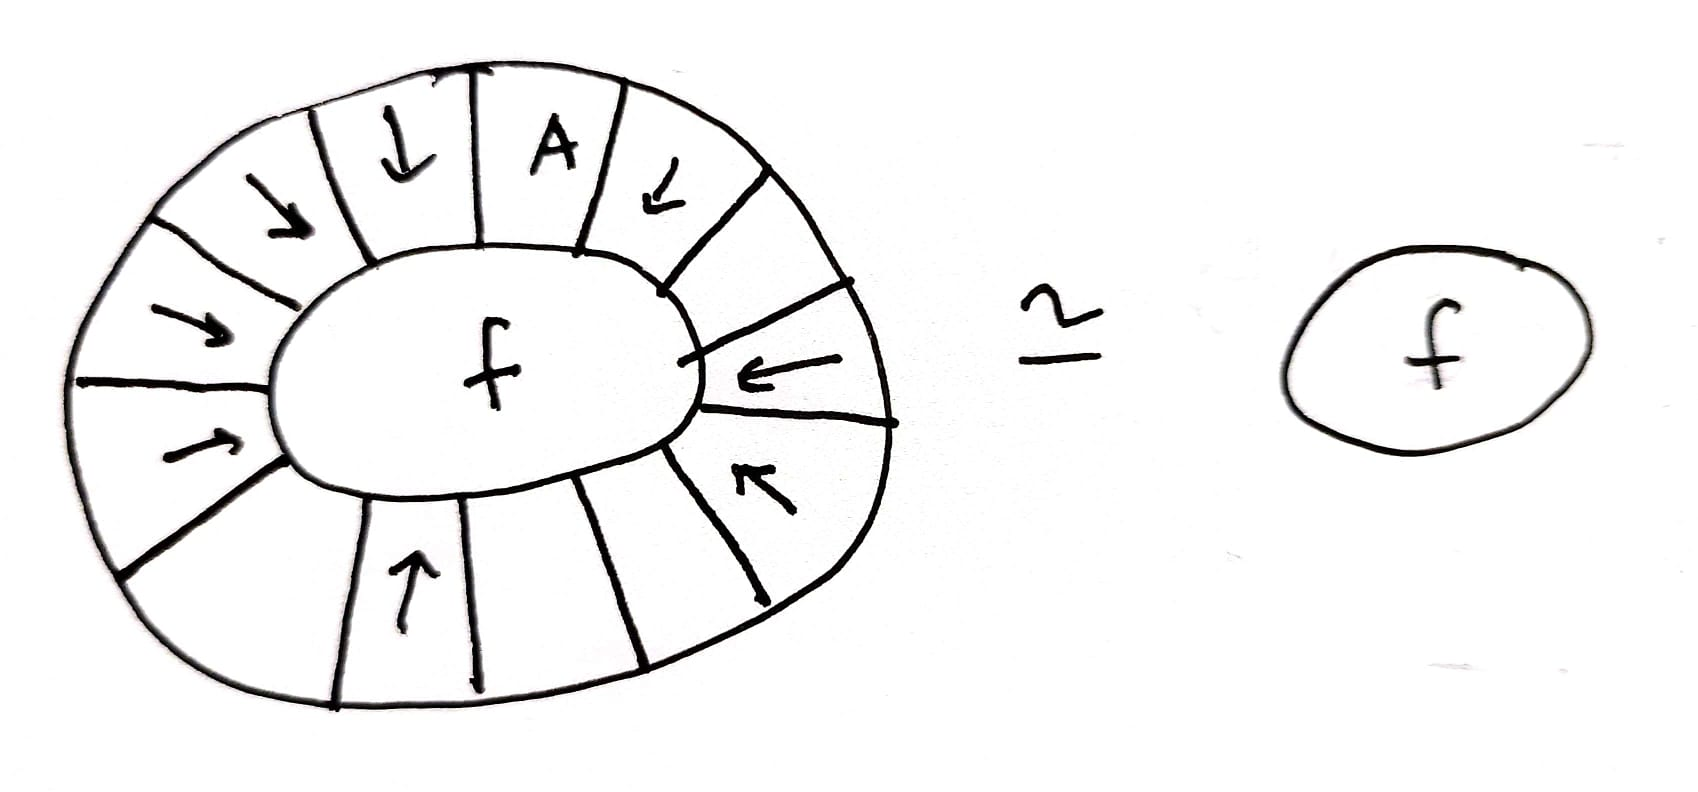
\includegraphics[width=0.6\textwidth]{Figures/p322.jpeg}
            \caption{}
            \label{fig:p322-jpeg}
        \end{figure}
        
        This shows that
        $r_* \circ j_* = \id$ which was what we wanted to show.\\
        \linebreak
        (3) Suppose
        \[
        1 \to A \stackrel{\alpha}{\to} B
        \stackrel{\beta}{\to} C \to 1
        \] 
        is a short exact sequence and
        let $s \colon B \to A$ be a retraction - i.e.,
        $s \circ \alpha = \id$.
        We claim that
        $\varphi \colon B \to A \times C$ by
        $\varphi (b) = \left( s(b),
        \beta(b)\right) $ is an isomorphism.
        Firstly, it is clearly a group homomorphism
        since $s$ and $\beta$ are assumed to be group homomorphisms.
        Next, for injectivity,
        if $\varphi (b) = 0$, then
        $s(b) = 0$ and $\beta(b) = 0$. But
        by exactness then there exists
        $a \in A$ such that $\alpha(a) = b$.
        Thus
        $a = \id (a)  = s \circ \alpha(a) 
        = s (b) = 0$. But then since
        $\alpha$ is a group homomorphism, it takes
        $0$ to $0$, so
        $b = \alpha(a) = \alpha(0) = 0$. This gives
        injectivity.\\
        For surjectivity, let
        $\left( a,c \right) \in A \times C$.
        Since $\beta$ is surjective by exactness of the SES,
        there exists $b \in B$ such that
        $\beta (b) = c$. Then
        $s (\alpha(a) - \alpha \circ s(b) +  b) =
        a - s(b) + s(b) = a$ while
        $\beta \left( \alpha(a) -
        \alpha \circ s(b) + b\right) 
        = \beta(b) = c$ since
        $\beta \circ \alpha = 0$. Hence
        $\varphi \left( \alpha(a - s(b))
         + b\right) = \left( a,c \right) $, so
         $\varphi $ is also surjective.\\
         To conclude the desired isomorphism of
         the problem, we simply note that
         by (1) and (2), we precisely have
         an exact sequence where
         $j_*$ admits a retraction, so
         by (3), we get an isomorphism
         \[
         \pi_n \left( X,A,x_0 \right) 
         \cong \pi_n (X,x_0) \times 
         \pi_{n-1}(A,x_0).
         \] 
    \end{proof}


